\documentclass{beamer}
\usepackage{inconsolata}
\usepackage{caption}
\usepackage{color}
\usepackage{listings}
\usepackage{subfig}
\usepackage{cooltooltips}
\usepackage{hyperref}
\usepackage{perpage}
\usepackage{graphics}
\usepackage{grffile}
\usepackage{kotex}
\usepackage[normalem]{ulem}
\setbeamertemplate{navigation symbols}{}%remove navigation symbols
\usepackage{listings}
\usepackage{color}
\usepackage{framed}

\definecolor{background}{RGB}{39, 40, 34}
\definecolor{string}{RGB}{230, 219, 116}
\definecolor{comment}{RGB}{117, 113, 94}
\definecolor{normal}{RGB}{248, 248, 242}
\definecolor{identifier}{RGB}{166, 226, 46}



\lstset{
  language=C,               			% choose the language of the code
  alsolanguage=Python,            			% choose the language of the code
  alsolanguage=Java,            			% choose the language of the code
  numbers=none,                   		% where to put the line-numbers
  stepnumber=1,                   		% the step between two line-numbers.        
  numbersep=5pt,                  		% how far the line-numbers are from the code
  extendedchars=true,
  numberstyle=\tiny\color{black}\ttfamily,
  backgroundcolor=\color{background},  		% choose the background color. You must add \usepackage{color}
  showspaces=false,               		% show spaces adding particular underscores
  showstringspaces=false,         		% underline spaces within strings
  showtabs=false,                 		% show tabs within strings adding particular underscores
  frame=single,
  framerule=0pt,
  tabsize=4,                      		% sets default tabsize to 2 spaces
  captionpos=n,                   		% sets the caption-position to bottom
  breaklines=true,                		% sets automatic line breaking
  breakatwhitespace=true,         		% sets if automatic breaks should only happen at whitespace
  title=\lstname,                 		% show the filename of files included with \lstinputlisting;
  basicstyle=\color{normal}\tiny\ttfamily,					% sets font style for the code
  keywordstyle=\color{magenta}\tiny\ttfamily,	% sets color for keywords
  stringstyle=\color{string}\tiny\ttfamily,		% sets color for strings
  commentstyle=\color{comment}\tiny\ttfamily,	% sets color for comments
  emph={True, False, format_string, eff_ana_bf, permute, eff_ana_btr, KeyError,
  ValueError, ZeroDivisionError},
  emphstyle=\color{identifier}\tiny\ttfamily,
  morekeywords={with, as}
}

\lstset{literate=%
   *{0}{{{\color{cyan}0}}}1
    {1}{{{\color{cyan}1}}}1
    {2}{{{\color{cyan}2}}}1
    {3}{{{\color{cyan}3}}}1
    {4}{{{\color{cyan}4}}}1
    {5}{{{\color{cyan}5}}}1
    {6}{{{\color{cyan}6}}}1
    {7}{{{\color{cyan}7}}}1
    {8}{{{\color{cyan}8}}}1
    {9}{{{\color{cyan}9}}}1
}



\newenvironment{enum}{
\begin{enumerate}
  \setlength{\itemsep}{1pt}
  \setlength{\parskip}{0pt}
  \setlength{\parsep}{0pt}
}{\end{enumerate}}

\hypersetup{
  colorlinks=true,
  urlcolor=pink,
}

\MakePerPage{footnote}

\title{파이썬 101}
\subtitle{무한한 라이브러리, 저 너머로!}

\begin{document}
\frame{\titlepage}

\begin{frame}
\frametitle{51일 전: 왜 파이썬?}
\begin{figure}[H]
  \centering
  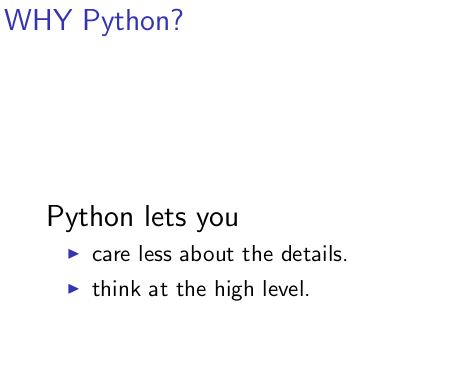
\includegraphics[width=80mm,height=60mm]{recap.png}
\end{figure}
공감 되시나요?
\end{frame}

\begin{frame}
  \frametitle{오늘: 왜 파이썬?}
\begin{figure}[H]
  \centering
  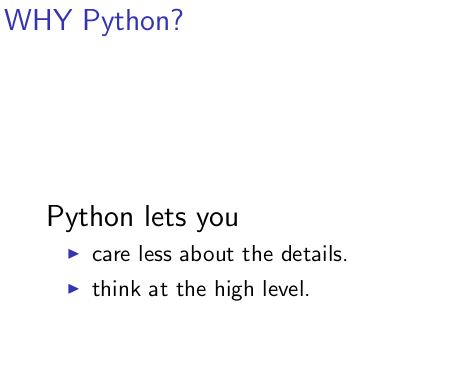
\includegraphics[width=80mm,height=60mm]{recap.png}
\end{figure}
  그리고 다양한 라이브러리들
\end{frame}

\begin{frame}
\frametitle{파이선이 슈퍼히어로라면\ldots}
\begin{figure}[H]
  \centering
  
\includegraphics[width=80mm,height=50mm]{hero.png}
\end{figure}
\end{frame}

\begin{frame}[fragile]
\frametitle{근데 진짜임}
\begin{lstlisting}
import antigravity
\end{lstlisting}
\end{frame}

\begin{frame}
\frametitle{유용한 모듈, 라이브러리와 프로그램들 일부}
\begin{itemize}
\item pdb: 디버깅\\
\item PyPy: 빠른 파이선\\
\item pip: 파이선 패키지 관리자\\
\item Numpy: 빠른 계산\\
\item Pillow: 이미지 처리\\
\item OpenCV: 컴퓨터 비전\\
\item Request: HTTP 요청 주고받기\\
\item Scrapy: 웹크롤링\\
\item Selenium: 웹브라우저 자동화\\
\item KoNLPY: 한국어 처리\\
\item tossi: 한국어 조사처리\\
\item Ren'Py: 비주얼 노벨 \footnotesize\sout{미연시} \normalsize만들기\\
\item Pygame: 2D 게임 만들기\\
\end{itemize}
\end{frame}

\begin{frame}{pdb}
  The Python Debugger
\end{frame}

\begin{frame}[fragile]{지금까지의 디버깅}
\begin{lstlisting}
def wrong_function(n):
    if n == 2 and n == 3:
      print("n is: ", n)
      return True
    if n % 2 == 0 or n < 2:
      print("n is now: ", n)
      return False
    for i in range(3,int(n**0.5+1),2):
        print(n, i)
        if n % i == 0:
            return False
        print("should not print if n is prime", i)
    if n == 3:
      print("if I can read this, I am XXXXed")
    return True
\end{lstlisting}
\end{frame}

\begin{frame}[fragile]{좋은 디버깅}
\begin{figure}[H]
  \centering
  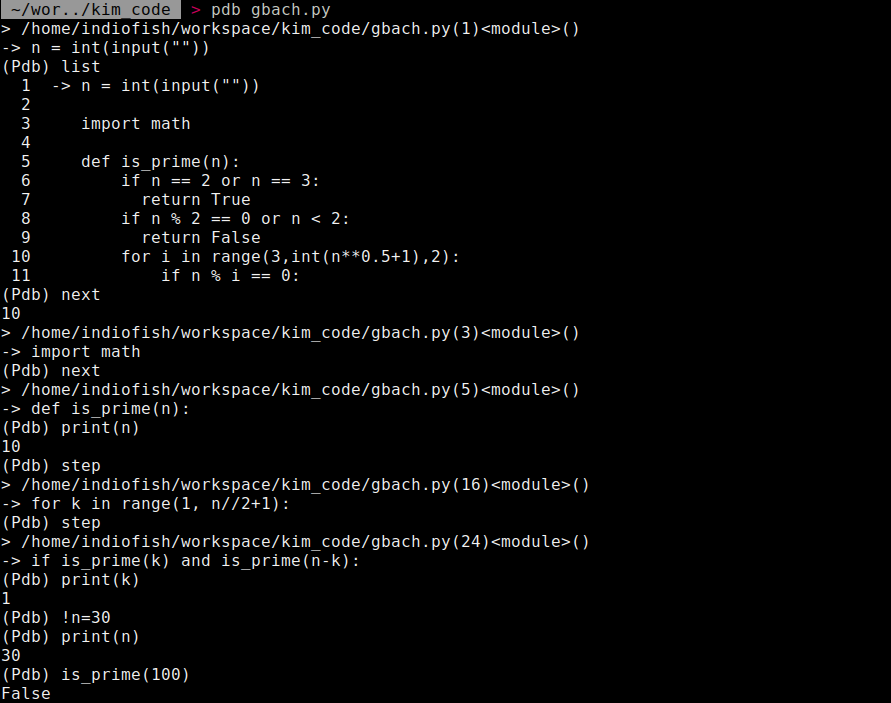
\includegraphics[width=100mm,height=75mm]{pdb_usage.png}
\end{figure}
\end{frame}

\begin{frame}{좋은 디버깅}
\begin{itemize}
  \item help\\
    가능한 명령어를 보여준다.
  \item break (줄번호$\vert$함수이름)\\
    n번째 줄이나 함수에 도달하면 일시정지
  \item print()\\
    우리가 아는 출력함수
  \item !x = 3\\
    값 바꾸기
  \item next\\
    현재 함수의 다음줄로 넘어간다.(중간의 함수는 그냥 실행)
  \item step\\
    step into: 함수 안으로 들어간다.
\end{itemize}
\end{frame}

\begin{frame}{좋은 디버깅}
장점들
\begin{itemize}
  \item 프로그램을 껐다켰다하지 않고도 테스트 가능
  \item 프로그램을 바꾸지 않고도 테스트 가능
  \item 멋있음
\end{itemize}
\end{frame}

\begin{frame}{PyPy}
\begin{figure}[H]
  \centering
  
\includegraphics[width=80mm,height=20mm]{pypy-logo.png}
\end{figure}
  Python으로 실행하는 Python
\end{frame}

\begin{frame}{PyPy}
  python program.py == pypy program.py\\
  JIT 컴파일과 파이선 코드를 C로 번역하는 과정 등을 거쳐 표준 python 구현체보다
  2-10배 정도 빠를 때도 있고, 조금 느릴 때도 있습니다.
\end{frame}

\begin{frame}{pip}
\textit{pip install you-name-it}\\
  파이썬에 기본적으로 포함되어 있는, 패키지 관리자. 일일이 홈페이지에 들어가서
  설치파일을 받지 않아도 되는 장점이 있습니다.
\end{frame}

\begin{frame}{Numpy}
\textit{pip install numpy}\\
Anaconda 등에 포함되어 있어 써보셨을 것 같은 Numpy\\
\end{frame}

\begin{frame}{왜 Numpy?}
  딥러닝 등의 근간이 되는 행렬\footnote{김모 교수님 \textit{"미적분학은 한물갔고 이젠 선형대수학의
  시대입니다 음하하!"}}을 빠르게 계산 해줍니다.
물론 그외에도 많은 수학기능이 있습니다.
\end{frame}

\begin{frame}[fragile]{Numpy}
\begin{lstlisting}
import numpy as np
SIZE = 500
a = np.array([[randint(-100,100) for _ in range(SIZE)] for _ in range(SIZE)])
b = np.array([[randint(-100,100) for _ in range(SIZE)] for _ in range(SIZE)])
c = np.dot(a, b)
\end{lstlisting}
500 x 500 행렬의 곱셈
\end{frame}

\begin{frame}[fragile]{Numpy vs 저}
\begin{figure}[H]
  \centering
  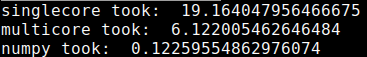
\includegraphics[width=75mm,height=20mm]{./numpy-result.png}
\end{figure}
코드는 깃 저장소의 mat\_mul.py에서 확인 가능합니다.
\end{frame}


\begin{frame}{Pillow}
\textit{pip install Pillow}\\
Python Image Library (PIL)의 변형판\\
사진을 늘리고, 줄이고, 변형하는데 유용합니다.\\
https://pillow.readthedocs.io/en/stable/
\end{frame}

\begin{frame}{Pillow}
  \begin{lstinputlisting}
    {pil_test.py}
  \end{lstinputlisting}
\end{frame}

\begin{frame}{OpenCV}
\textit{pip install opencv-python}\\
https://docs.opencv.org/master/d6/d00/tutorial_py_root.html\\
이미지처리 + 컴퓨터비전을 위한 라이브러리.\\
Pillow보다 강력하지만, 복잡하네요\\
컴퓨터비전 이론을 몰라도 Ctrl CV로 사용할 수 있으나, 왜 결과가 나오는 지 모를 수가 있음.
\end{frame}

\begin{frame}{심슨}
\begin{figure}[H]
  \centering
  
\includegraphics[width=100mm,height=60mm]{simpsons.jpeg}
\end{figure}
\end{frame}

\begin{frame}{누구 눈일까요? 5초}
\begin{figure}[H]
  \centering
  
\includegraphics[width=20mm,height=20mm]{eyes3.jpeg}
\end{figure}
\end{frame}

\begin{frame}{OpenCV - Template Matching Ctrl CVed}
\begin{lstinputlisting}
  {cv_test.py}
\end{lstinputlisting}
\end{frame}

\begin{frame}{아하.}
\begin{figure}[H]
  \centering
  
\includegraphics[width=100mm,height=60mm]{res.png}
\end{figure}
\end{frame}

\begin{frame}{Requests}
\begin{lstinputlisting}
  {cv_test.py}
\end{lstinputlisting}
\end{frame}

\begin{frame}{Requests}
\textit{pip install requests}\\
HTTP 요청\footnote{비약하자면, 인터넷}을 주고받는 모듈\\
https://2.python-requests.org/en/master/
\end{frame}

\begin{frame}{족보를 구하러 가자}
이 페이지를 보여주는 HTML문서에서 숫자 이미지의 위치를 찾을 수 있습니다. src의 주소에서 이미지를 다운 받는 것
  같네요.
\end{frame}

\begin{frame}{족보를 구하러 가자}
  링크를 우클릭해서 복사(Copy link address)해봅시다. 주소는 사람마다 다를 수
  있습니다. 
\end{frame}

\begin{frame}{문제은행이 여기있네}
  짠! 복사한 링크를 크롬에서 열어보면, 새로고침 할 때마다 새로운 숫자캡챠가 나오는 
  페이지가 나옵니다.
\end{frame}

\begin{frame}{웹크롤링 등판}
  이젠 웹크롤링을 이용해서 저 링크에서 사진을 여러 장 다운받으면, 날 것의
  데이터는 준비가 끝납니다.
\end{frame}

\begin{frame}{웹크롤링 등판}
  아까의 링크로부터 IMG\_COUNT 만큼 사진을 다운받는 코드입니다. 너무 많이 접속하면 수상하니깐,
  $time.sleep()$ 으로 조금 기다립니다.
\end{frame}

\begin{frame}{제 2 장}
  데이터 요리하기
\end{frame}

\begin{frame}{날 것의 데이터}
 확보한 500장의 숫자 데이터는 여러가지 문제점이 있습니다.
  \begin{enumerate}
    \item 여러가지 색깔이다.\\
      컴퓨터가 색깔이 다른 같은 숫자를 다른 것으로 인식한다면, 학습시키기가
      어렵습니다.
    \item 두 자리 숫자이다.\\
      0-9는 10개만 구분하면 되지만, 10-99 는 90개를 구분해야 합니다. 
    \item 해답이 없다.\\
      기출문제에 답이 있어야 공부가 되겠죠? 지금의 데이터는 라벨링이 되지
      않아서, 컴퓨터가 학습을 하더라도 뭐가 뭔지 알 수가 없습니다.
  \end{enumerate}
\end{frame}

\begin{frame}{날 것의 데이터}
  쉬운 문제점들부터 해결합니다.
  \begin{enumerate}
    \item 여러가지 색깔이다.\\
      이미지 처리를 통해 사진을 흑백으로 바꾸면 됩니다.
    \item 두 자리 숫자이다.\\
      흑백으로 바꾼 후에는, 바탕과 숫자의 경계를 쉽게 구분하여, 숫자들을 한
      자리씩 쉽게 분리 할 수 있습니다.
  \end{enumerate}
\end{frame}

\begin{frame}{데이터 요리하기}
  이미지 처리를 위해서는 OpenCV를 활용합시다.
\end{frame}

\begin{frame}{데이터 요리하기}
  이미지 처리를 위해서는 OpenCV를 활용합시다.
\end{frame}

\begin{frame}{데이터 요리하기}
  gray image, 즉 흑백으로 바꿔주는 부분입니다.
\end{frame}

\begin{frame}{데이터 요리하기}
  Contour는 이미지에서 끊기지 않고 연결되어 있는 부분을 말합니다.
  두 숫자겠지요. boundingRect는 그 부분을 감싸는 최외곽 직사각형을 의미합니다.
  데이터에서 2개의 boundingRect를 추출하여, 숫자 2개를 분리할 수 있습니다.
\end{frame}

\begin{frame}{데이터 요리하기-사소하지만 중요한}
  숫자의 크기가 다르면, 학습시키는 것이 귀찮거나, 불가능 할 수도 있습니다.
  적절한 보간법(INTER\_CUBIC)을 이용해 각기 다른 크기의 숫자들을 28x28로
  통일시켜줍니다.
\end{frame}

\begin{frame}{데이터 요리하기- 초벌 끝}
  1000장의, 동일한 크기의, 흑백 숫자 이미지를 얻었습니다. 각 숫자 당 약 100장
  씩 입니다.
\end{frame}

\begin{frame}{데이터 요리하기- 어려운 부분}
  \begin{enumerate}
    \item 해답이 없다.\\
      학습 데이터에 한해서는, 사람이 직접 정답이 뭔지 적어주어야 합니다.
      성능이 떨어지는 알고리즘의 도움을 받아
      라벨링을 할 때도 있으나, 결국 사람이 확인해야 합니다.
      기계학습 연구실 대학원생의 존재의의입니다.\\
  \end{enumerate}
\end{frame}

\begin{frame}{데이터 요리하기}
  그럼, 이제 1000개의 숫자를 맞춰 줄 대학원생을 구하기 위해 교수가 되어봅시다.
\end{frame}

\begin{frame}{데이터 요리하기}
  도와주는 스크립트: 숫자 이미지를 화면에 띄워주고, 무슨 숫자인지
  입력하면 파일명(라벨)을 바꿔줍니다.
\end{frame}

\begin{frame}{오늘은 내가 대학원생}
\end{frame}

\begin{frame}{요리준비 끝}
2시간 정도 걸렸습니다.
\end{frame}

\begin{frame}{예고}
잘 정제된 자료를 확보하였으니, 적절한 기계학습 알고리즘을 골라 학습시킵니다.
그후에, 수강신청사이트에서 직접 이미지를 캡쳐하고, 위의 방법대로 흑백으로
  만들고, 쪼개고, 크기를 바꾼 다음, 컴퓨터 보고 맞춰보라 합니다.
\end{frame}


\end{document}
